\section{Formulazas}

%=%=%=%=%=%=%=%=%=%=%=%=%=%=%=%=%=%=%=%=%=%=%=%=%=%=
%=%=%=%=%=%=%=%=%=%=%=%=%=%=%=%=%=%=%=%=%=%=%=%=%=%=
\subsection{Lógica - Conjuntos - Bitwise}
$\oplus$ es el xor (o diferencia simétrica de conjuntos).
\begin{enumerate}[1.]
    \item $a|b = a\oplus b + a \& b$
    \item $a\oplus (a\&b) = (a|b)\oplus b$
    \item $b\oplus (a\&b) = (a|b)\oplus a$
    \item $(a\&b)\oplus (a|b) = a\oplus b$
    \item $a + b = a|b + a\&b = a\oplus b + 2(a\&b)$
    \item $a - b = (a\oplus (a\&b))-((a|b)\oplus a) = ((a|b)\oplus b)-((a|b)\oplus a)$
    \item $a - b = (a\oplus (a\&b))-(b\oplus (a\&b)) = ((a|b)\oplus b)-(b\oplus (a\&b))$
\end{enumerate}

Si $p, q$ son predicados, entonces:
\begin{enumerate}[1.]
    \item $(p \vee q) \iff -(-p \wedge -q)$.
    \item $(p \implies q) \iff (-p \vee q)$.
    \item $(p \oplus q) \iff -(p \iff q)$.
\end{enumerate}

\subsection{Combinatoria}

\textbf{Inclusión-Exclusión.} Sean $A_1, \dots, A_n$ conjuntos, entonces
$$\abs{\bigcup_{i = 1}^n A_i} = \sum_{\varnothing \neq J \subseteq [n]} (-1)^{|J| - 1}\abs{\bigcap_{j \in J} A_j}$$

\textbf{Cantidad de elementos en exactamente $r$ conjuntos.} Sean $A_1, \dots, A_n$ conjuntos y $0 \leq r \leq n$, la cantidad de elementos en exactamente $r$ conjuntos $A_i$ es
$$\sum_{m = r}^n (-1)^{m - r}\binom{m}{r}\sum_{\substack{J \subseteq [n]\\|J| = m}} \abs{\bigcap_{j \in J} A_j}$$

\textbf{Teorema del binomio generalizado.} Para $x \in \R$ y $a, b \in \mathbb{C}$ se cumple
$$(a + b)^x = \sum_{k = 0}^\infty \binom{x}{k}a^{x}b^{x - k},$$
$$\binom{x}{k} = \frac{1}{k!}\prod_{j = 0}^{k - 1}(x - j) = \frac{x(x - 1)(x - 2)\cdots(x - k + 1)}{k!}.$$

\textbf{ES FIBONACCI} \textit{(En un icpc, el de la Cangurera lo usó)}. En el \textit{Triángulo de Pascal}, los elementos en una ``diagonal'' satisfacen
\[
F_{n+1} = \sum_{k=0}^{\lfloor n/2 \rfloor} \binom{n-k}{k},
\]
donde \( F_{n+1} \) es el \((n+1)\)-ésimo número de Fibonacci.

\begin{figure}[H]
    \centering
	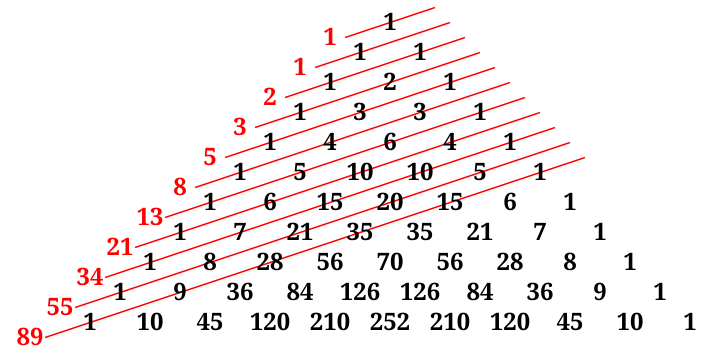
\includegraphics[width=0.5\columnwidth]{img/FiboPascal.png}
\end{figure}

\textbf{Palo de Hockey.}
Para \( n \) y \( r \) \((n \geq r)\), se cumple
\[
\sum_{k=r}^{n} \binom{k}{r} = \binom{n+1}{r+1}.
\]

\textbf{Derangements.} ¿Cuántos trastornos mentales distintos de tamaño $n$ hay? (Según Google Translator). Considera los conjuntos $\set{A_k}_{k = 1}^{k = n}$ donde $A_k$ es la cantidad de permutaciones con el punto fijo $p_k = k$. La cantidad de permutaciones con al menos un punto fijo es
\begin{align*}
	P &:= \abs{\bigcup_{i = 1}^n A_i} = \sum_{\varnothing \neq J \subseteq [n]} (-1)^{|J| - 1}\abs{\bigcap_{j \in J} A_j}\\
	&= \sum_{\varnothing \neq J \subseteq [n]} (-1)^{|J| - 1}(n - |J|)!
	= \sum_{i = 1}^n (-1)^{i - 1}\binom{n}{i}(n - i)!,
\end{align*}

entonces la cantidad de desarreglos es $n! - P$. Si $d_n$ es la cantidad de desarreglos de tamaño $n$ se cumple $d_n = (n - 1)(d_{n  -1} + d_{n - 2})$ con $d_1 = 0$ y $d_0 = d_2 = 1$. También se cumple $d_n = n!d_{n - 1} + (-1)^n$. Sea $0 \leq k \leq n$ y $d_{n, k}$ la cantidad de desarreglos de tamaño $n$ con exactamente $k$ puntos fijos, entonces $d_{n, k} = \binom{n}{k}d_{n - k}$.

%=%=%=%=%=%=%=%=%=%=%=%=%=%=%=%=%=%=%=%=%=%=%=%=%=%=
%=%=%=%=%=%=%=%=%=%=%=%=%=%=%=%=%=%=%=%=%=%=%=%=%=%=
\subsection{Geometría}

\textbf{Teorema de los círculos de Descartes}. Si cuatro círculos son mutuamente tangentes de curvatura $k_i= 1/r_i$ el teorema dice:
\begin{equation*}
    (k_1+k_2+k_3+k_4)^2 = 2\left( k_1^2 +k_2^2 +k_3^2 +k_4^2   \right)
\end{equation*}
\begin{equation*}
    k_4 = k_1+k_2+k_3 \pm 2\sqrt{k_1k_2+k_2k_3+k_3k_1}
\end{equation*}

\textbf{Formula de Heron}. Dado un trinangulo de lados $a, b, c$, escribimos su semiperimetro $s = \frac{a+b+c}{2}$, inradio r, y cuirunradio R.

\begin{equation*}
    Area = \sqrt{s(s-a)(s-b)(s-c)}
\end{equation*}
\begin{equation*}
    2R = \frac{abc}{2  \sqrt{s(s-a)(s-b)(s-c)}}
\end{equation*}
\begin{equation*}
    r =  \sqrt{\frac{(s-a)(s-b)(s-c)}{s} }
\end{equation*}

\textbf{Fórmula de Brahmagupta}. Para el Area se vale algo similar en cuadrilateros ciclicos
\begin{equation*}
    Area = \sqrt{(s-a)(s-b)(s-c)(s-d)}
\end{equation*}

Para no cíclicos, $\theta=$ promedio de dos ángulos opuestos, $p$ y $q$ diagonales
\begin{align*}
    Area &= \sqrt{(s-a)(s-b)(s-c)(s-d)-abcd \cos^2\theta}\\
    &=\sqrt{K},
\end{align*}

donde $K = (s-a)(s-b)(s-c)(s-d) - \frac{1}{4}(ac+bd+pq)(ac+bd-pq)$.

\textbf{Multidimensional} \textit{(Como Chang).} Para más dimensiones, si $A$ es la matriz con filas estos vectores
\begin{equation*}
    Volumen_n = \frac{1}{n!} \sqrt{det\Pa{AA^T}}
\end{equation*}